\documentclass[border={10pt, 10pt, 10pt, 10pt}]{standalone}

\usepackage{tikz}
\usepackage{graphicx}
\usepackage{varwidth}

\renewcommand\familydefault{\sfdefault}

\begin{document}
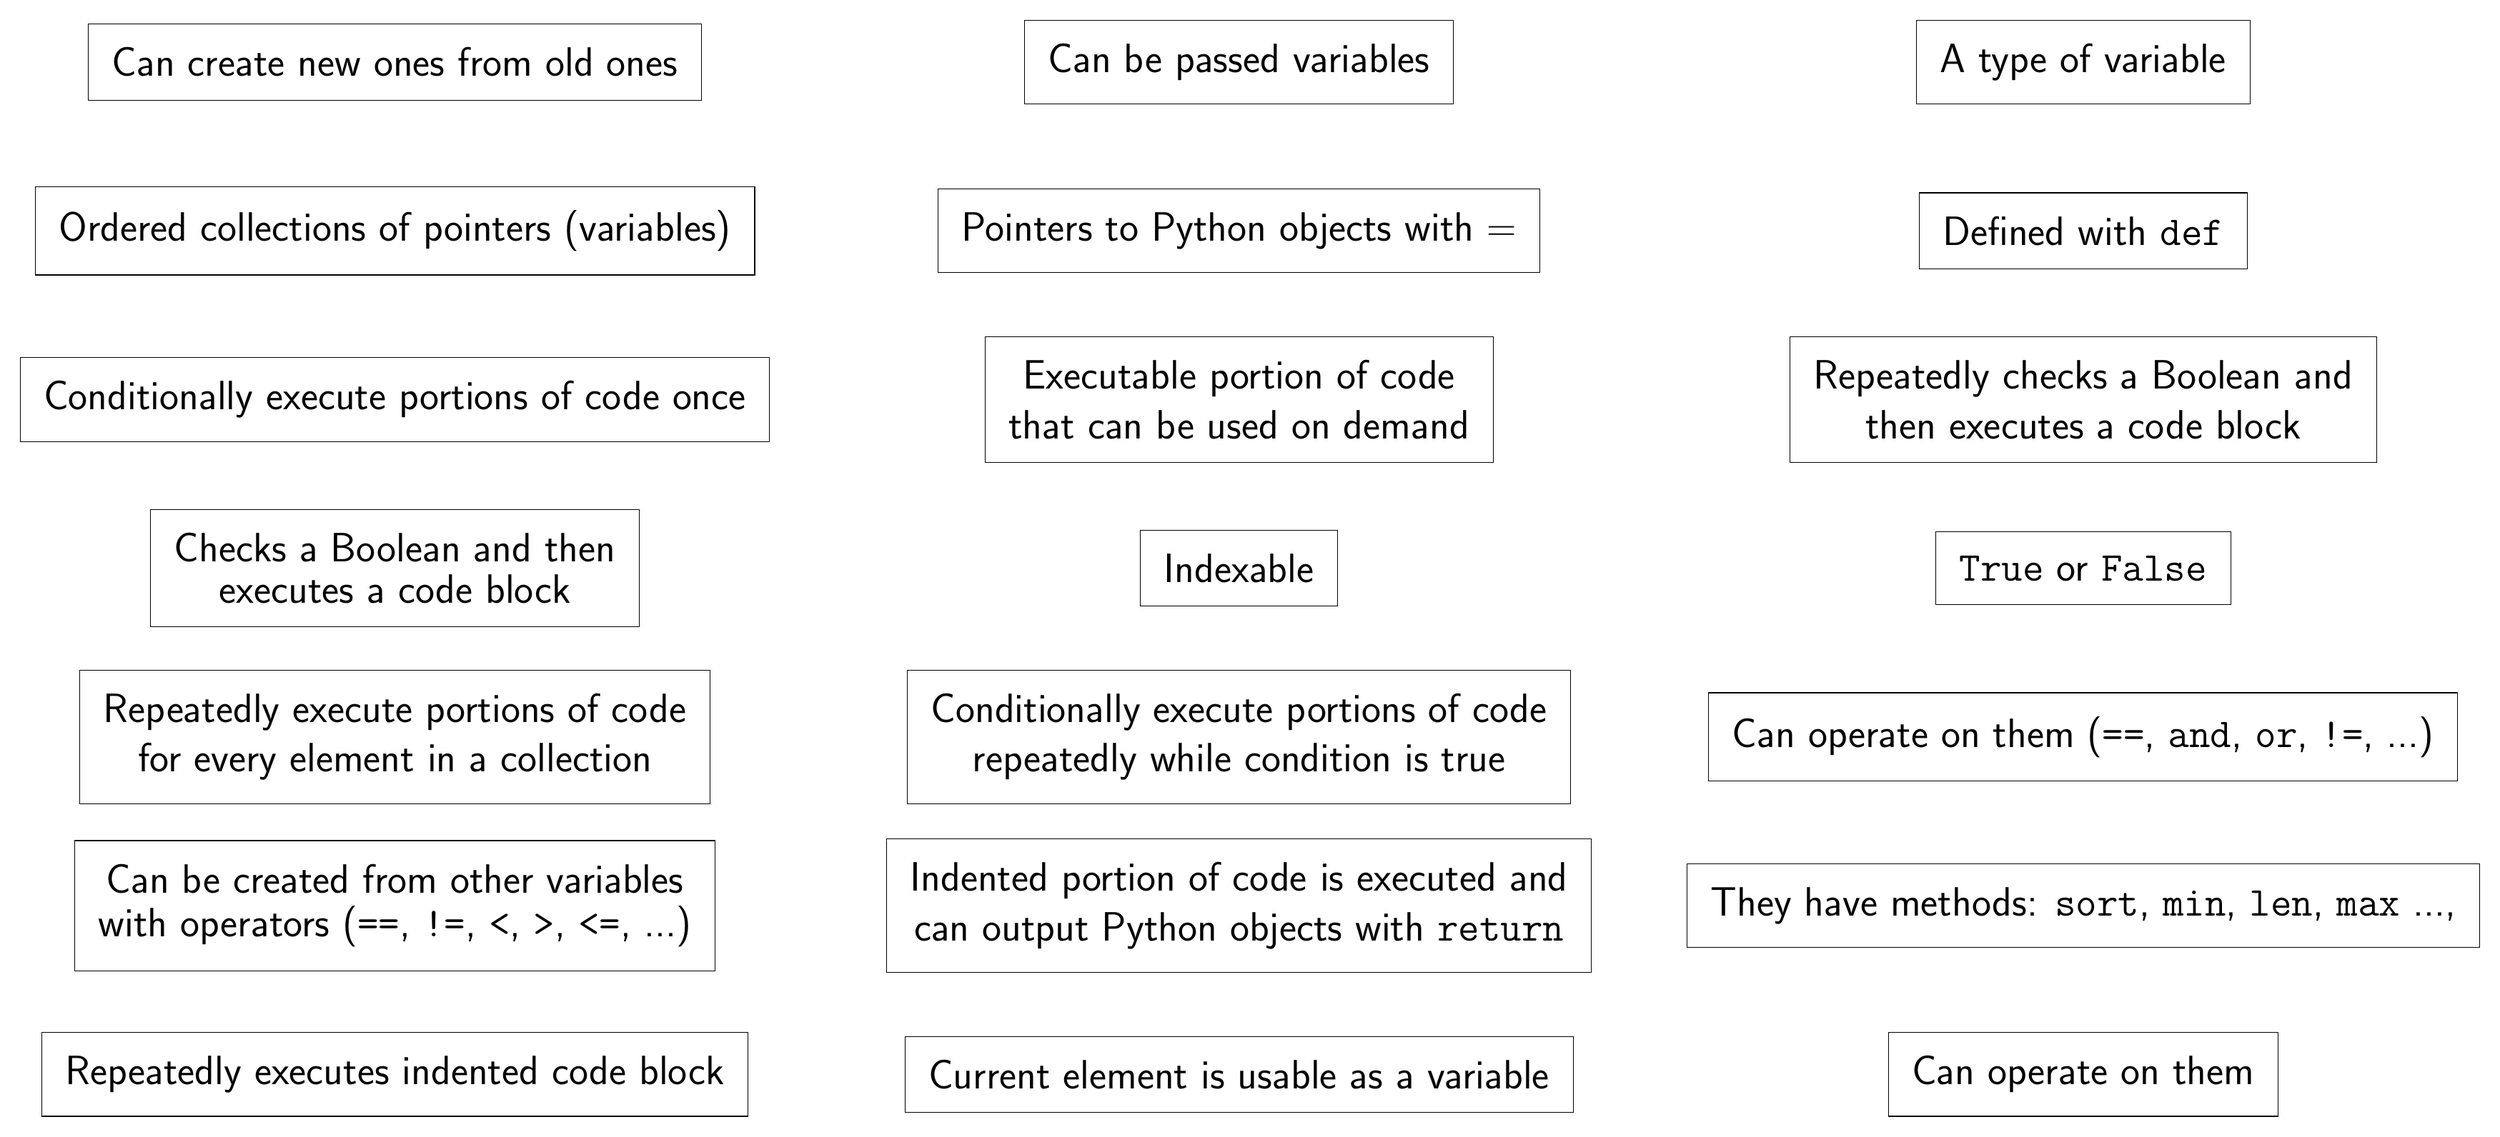
\begin{tikzpicture}
\node[align=center, draw=black, inner sep=12] at (0, 0) {\huge Repeatedly executes indented code block};
\node[align=center, draw=black, inner sep=12] at (15, 0) {\huge Current element is usable as a variable};
\node[align=center, draw=black, inner sep=12] at (30, 0) {\huge Can operate on them};
\node[align=center, draw=black, inner sep=12] at (0, 3) {\huge Can be created from other variables\\[2mm]\huge with operators (\texttt{==}, \texttt{!=}, \texttt{<}, \texttt{>}, \texttt{<=}, ...)};
\node[align=center, draw=black, inner sep=12] at (15, 3) {\huge Indented portion of code is executed and\\[2mm]\huge can output Python objects with \texttt{return}};
\node[align=center, draw=black, inner sep=12] at (30, 3) {\huge They have methods: \texttt{sort}, \texttt{min}, \texttt{len}, \texttt{max} ...,};
\node[align=center, draw=black, inner sep=12] at (0, 6) {\huge Repeatedly execute portions of code\\[2mm]\huge for every element in a collection};
\node[align=center, draw=black, inner sep=12] at (15, 6) {\huge Conditionally execute portions of code\\[2mm]\huge repeatedly while condition is true};
\node[align=center, draw=black, inner sep=12] at (30, 6) {\huge Can operate on them (\texttt{==}, \texttt{and}, \texttt{or}, \texttt{!=}, ...)};
\node[align=center, draw=black, inner sep=12] at (0, 9) {\huge Checks a Boolean and then\\[2mm]\huge executes a code block};
\node[align=center, draw=black, inner sep=12] at (15, 9) {\huge Indexable};
\node[align=center, draw=black, inner sep=12] at (30, 9) {\huge \texttt{True} or \texttt{False}};
\node[align=center, draw=black, inner sep=12] at (0, 12) {\huge Conditionally execute portions of code once};
\node[align=center, draw=black, inner sep=12] at (15, 12) {\huge Executable portion of code\\[2mm]\huge that can be used on demand};
\node[align=center, draw=black, inner sep=12] at (30, 12) {\huge Repeatedly checks a Boolean and\\[2mm]\huge then executes a code block};
\node[align=center, draw=black, inner sep=12] at (0, 15) {\huge Ordered collections of pointers (variables)};
\node[align=center, draw=black, inner sep=12] at (15, 15) {\huge Pointers to Python objects with $=$};
\node[align=center, draw=black, inner sep=12] at (30, 15) {\huge Defined with \texttt{def}};
\node[align=center, draw=black, inner sep=12] at (0, 18) {\huge Can create new ones from old ones};
\node[align=center, draw=black, inner sep=12] at (15, 18) {\huge Can be passed variables};
\node[align=center, draw=black, inner sep=12] at (30, 18) {\huge A type of variable};

\end{tikzpicture}
\end{document}